\chapter{Methodik}

> Validation Stage (= Kapitel „Vergleich der Browser“)

Warum Methodik? 
	> \cite{Aggarwal.2010}
		Aufgrund der Komplexität moderner Browser ist eine systematische Methode erforderlich, um zu testen, ob der private Browsing-Modus ausreichend gegen die Bedrohungsmodelle aus Abschnitt 2 verteidigt.		
	> \cite{Izzati.2022}
		•	Die Verfahren für die digitale Forensik für Browser-Forensik müssen angemessen befolgt werden, um dem Ermittler bei der Durchführung der Untersuchung zu helfen. Die Verfahren unterscheiden sich je nachdem, wie die Untersuchung durchgeführt werden soll.
	> \cite{Horsman.2019}
		•	Das Fehlen von Klarheit hat einen signifikanten Einfluss auf forensische Untersuchungen von Strafverfolgungsbehörden und deren Ansätze
		•	Eine Kette von Beweisführung muss dokumentiert werden, um die Integrität und Zuverlässigkeit der Daten sicherzustellen.
		•	Ein formaler forensischer Bericht wird dann vor Gericht präsentiert.
	
	
Bekanntes Computer Forensik Vorgehensmodell: \cite{Yusoff.2011}: Generic Model Computer Forensics Investigations (GCFIM) -> Daran orientieren sich alle in der Literatur

BSI: "abschnittsbasierter Verlauf einer forensischen Untersuchung" % https://www.bsi.bund.de/SharedDocs/Downloads/DE/BSI/Cyber-Sicherheit/Themen/Leitfaden_IT-Forensik.pdf?__blob=publicationFile&v=2
- Vorbereitung;
- Datensammlung;
- Untersuchung: Extraktion von Bilddateien aus dem Image
- Datenanalyse: Verbindungen zwischen mehreren Daten herstellen
- Dokumentation

Phasen nach \cite{Montasari.2015}
	•	Die forensische Analyse erfolgt in zwei Phasen.
	1.	Zunächst wird die Analyse an sowohl "üblichen" als auch "ungewöhnlichen" Speicherorten auf der Festplatte durchgeführt.
	2.	In der zweiten Phase wird der physische Arbeitsspeicher (RAM) untersucht.

Phasen nach \cite{Izzati.2022}:
	•	Es gibt verschiedene Modelle für digitale Forensik, die sich in ihren Phasen unterscheiden können.
	•	Fünf Phasen sind besonders wichtig: Identifikation und Sammlung, Bewahrung, Erwerb, Analyse und Prüfung sowie Dokumentation.
	•	In der Identifikations- und Sammelphase werden alle potenziellen Beweismittel identifiziert, gekennzeichnet und gesammelt, um sie in der nächsten Phase zu verwenden.
	•	Beweismittel können z.B. Log-Dateien, temporäre Dateien, Netzwerkverbindungen, Browserverlauf und Cache sein.
	> Phasen:
		Preparation Phase
		o	Versuchsplanung + Konfiguration der HW/SW + Durchführen des Experiments Acquisition Stage
		o	Abbildung von der Festplatte (Static Forensics) und des RAMs (Live Forensics) Analysephase
		o	Bilder der Speicherabbilder mit einem forensischen Tool untersuchen	Validierungsphase
		o	gefundenen Artefakte verglichen und dokumentiert

\section{Vorbereitung}

- \cite{Izzati.2022} Versuchsplanung + Konfiguration der HW/SW + Durchführen des Experiments Acquisition Stage
- BSI: alle Maßnahmen, die nach vermuteten Eintreten eines Vorfalls aber vor der eigentlichen Datensammlung erfolgen. 
	-> z.B. Identifikation und Enumeration potentieller Datenquellen

\subsection{Browserauswahl}

> Browserstudie \cite{Izzati.2022}
- Die Herstellerangaben unterschiedlicher Browser bzgl. Privatheit untersucht
- Firefox 58.02: No Browsing History stored, No Cookies stored, No login Info stored, Tracking Protection Enabled: Disconnect, Download Files not Hidden
- Chrome 63.0.3239: No Browsing History stored, No Cookies stored, No login Info stored, Tracking Protection Enabled: No, Download Files not Hidden

> design aim of Tor: \cite{Muir.2019}
- preventing from writing to disk (Perry et al., 2018) 
- enabling secure deletion of the browser (Sandvik, 2013) (hier nicht relevant)

\subsection{Browsing Szenario}
- Wichtig für White-Box-Ansatz: Browsing Szenario ist bekannt
- URL X … 	(TODO!)
*** TODO: Automatisch geöffnete Firefox Seiten erwähnen ***
*** TODO: Hier auch Browser Artefakte (Strings) auflisten ***

\subsection*{VM Konfiguration}

Virtualisierung:
	> Oracle VirtualBox VM, Version 7.0.8 r156879 (Qt5.15.2)
	TODO: Warum Virtualisierung?
	> Pro Browser eine VM

VM Betriebssystem: In Literatur (wie viele?) ausschließlich Windows untersucht -> Da Ziel dieser Arbeit: keine neuen wissenschaftlichen Ergebnisse => auch Windows 10
	Dazu: Windows 10 Pro, Build: 19045.2006 (nicht aktiviert)
	> Auf einer VM installiert, danach OVA erstellt. Von dieser ausgehend, für jeden Browser VM erstellt

VM Massenspeicher: 30 GB (VDI-Format), kein SSD-Laufwerk

VM RAM: Kaum Angaben in der Literatur:
	> \cite{Rochmadi.2017}: 2 GB 
	> \cite{Ohana.2013}: 4 GB
	- Hier: 6 GB (maximal möglich, mit verfügbaren Speicherresourcen, um später RAM-Dumps zu speichern)
	-> Ausblick: Kritik an Literatur, dass RAM-Größe kaum thematisiert wird, obwohl sie Auswirkungen auf Ergebnisse hat -> Siehe Pagefile-Thematik in Analysis Stage

VM Netzwerkeinstellungen: An Literatur orientiert (Quelle?)
	- Netzwerkadapter mit Netzwerkbrücke = direkt mit dem physischen Netzwerk deines Hostsystems verbinden -> virtuelle Maschine eine eigene IP-Adresse im physischen Netzwerk
	- Netzwerkadapter erst nach Browserinstallation aktiviert

Programme auf VM:
*** TODO: Shared Folder für Installation ***
	- Untersuchter Browser. Installationsverzeichnisse:
		> Firefox: % C:\Program Files\Mozilla Firefox\firefox.exe
		> Tor: % "C:\Program Files\Tor Browser\Browser\firefox.exe"
		> Chrome:
		> Brave:
			
	- Process Monitor
		"Process Monitor ist ein Dienstprogramm für das Windows-Betriebssystem, das von Microsoft entwickelt wurde. Es ermöglicht die Überwachung und Aufzeichnung aller Aktivitäten und Ereignisse, die auf einem Windows-System im Zusammenhang mit Prozessen, Dateisystemen, Registrierungseinträgen, Netzwerkverbindungen und vielem mehr stattfinden. Mit Process Monitor kannst du detaillierte Informationen über den Betrieb deines Systems erhalten, um Probleme zu diagnostizieren, Softwarekonflikte zu lösen oder verdächtige Aktivitäten zu untersuchen. Das Tool bietet eine umfassende Echtzeit-Überwachungsfunktion, die es dir ermöglicht, alle Ereignisse und Aktionen zu erfassen, die während der Ausführung von Prozessen auf deinem System auftreten."
		% https://learn.microsoft.com/de-de/sysinternals/downloads/procmon
		Version: v3.93
		Hier: Verwendet, um Aktivitäten des Browsers aufzuzeichnen (vgl. Wireshark Capture) -> Siehe Sammlungsphase
	
	- Process Explorer
		"Process Explorer erweitert die Funktionen des Windows Task Managers und ermöglicht es Benutzern, einen umfassenden Überblick über alle aktiven Prozesse und deren Eigenschaften zu erhalten." 
		Hier wichtig: Ermöglicht zudem alle ausgeführten Services einer PID zuzuordnen
		% https://learn.microsoft.com/de-de/sysinternals/downloads/process-explorer
		Version: v17.04

\subsection{Analysewerkzeuge}

\subsubsection*{Volatility}

 % https://www.volatilityfoundation.org/
	"Das Volatility Memory Forensics Framework ist ein Open-Source-Tool, das für die forensische Analyse von Arbeitsspeicherabbildern verwendet wird. Es ist speziell darauf ausgerichtet, Informationen und Artefakte aus dem physischen oder virtuellen Arbeitsspeicher eines Computers zu extrahieren.
	
	Frei auf GitHub verfügbar: % https://github.com/volatilityfoundation/volatility3	
	Version: 2.4.1 (aktuellster Release)
	Basierend auf python

	Die Volatility Foundation wurde ins Leben gerufen, um die Interessen der Volatility-Community zu vertreten und sicherzustellen, dass das Framework frei verfügbar 	bleibt und kontinuierlich weiterentwickelt wird. Das Projekt wird von einer Gemeinschaft von Freiwilligen vorangetrieben, die zur Code-Entwicklung, Dokumentation und Fehlerbehebung beitragen.

	Das Tool wurde entwickelt, um Forensikern und Sicherheitsexperten bei der Untersuchung von Sicherheitsvorfällen, Malware-Angriffen und anderen verdächtigen Aktivitäten zu unterstützen. Durch die Analyse des Arbeitsspeichers können wichtige Informationen wie Prozesse, Netzwerkverbindungen, Dateisystemstrukturen, Registrierungseinträge und sogar verschlüsselte Daten wiederhergestellt werden."

	Volatility3:
	"Volatility 3 tatsächlich eine vollständige Neuschreibung des Volatility Memory Forensics Frameworks zu sein, die im Jahr 2020 veröffentlicht wurde. Diese Neuschreibung sollte viele technische und Leistungsprobleme der ursprünglichen Version beheben, die seit der ersten Veröffentlichung im Jahr 2007 aufgetreten sind.

	Volatility 3 wurde mit dem Ziel entwickelt, eine robustere, flexiblere und skalierbarere Plattform für die Analyse von Arbeitsspeicherabbildern bereitzustellen. Es wurden Verbesserungen hinsichtlich der Architektur, der Leistung und der Plugin-Entwicklung vorgenommen. Die Neuschreibung ermöglichte auch eine Anpassung der Lizenzierung durch die Einführung der Volatility Software License (VSL)."

	Großer Vorteil von Volatility3: kein "Profile" mehr notwendig. = Konfigurationseinstellung, die angibt, um welches Betriebssystem und welche Version es sich im Arbeitsspeicherabbild handelt. Ein Profil definiert die Speicherstruktur und die Verhaltensweisen des Betriebssystems, die Volatility bei der Analyse des Arbeitsspeichers berücksichtigen muss.
		=> Grund: kann neue Symboltabellen für die meisten Windows-Speicherabbilder generieren, basierend auf dem Speicherabbild selbst
		% https://volatility3.readthedocs.io/en/latest/vol2to3.html

	Plugins-Liste: (Ähnlich zu \cite{Hariharan} und \cite{Dayalamurthy.2013})
	  > pslist	
	  > yarascan		
	  > memmap	 	
	  > filescan
	  > svcscan
		
	Genaue Beschreibung der PlugIns und deren Zusammenhang: Siehe Analysephase		
	Zusammenhang der Plugins: Siehe Analysephase

\subsubsection*{Autopsy}
	"Autopsy ist ein Open-Source-Digital-Forensik-Tool, das auf der Sleuthkit-Bibliothek basiert. Es wurde entwickelt, um forensische Untersuchungen von digitalen Beweismitteln auf Computern und mobilen Geräten durchzuführen.

	Sleuthkit ist eine Sammlung von Open-Source-Tools für die forensische Analyse von Dateisystemen. Es bietet Funktionen zum Lesen, Analysieren und Wiederherstellen von Daten aus verschiedenen Dateisystemen, darunter NTFS, FAT, exFAT, HFS+, Ext2/3/4 und mehr. Sleuthkit ermöglicht die Extraktion von Metadaten, das Durchsuchen von Dateien und die Analyse von Dateisystemstrukturen, um wichtige Informationen für forensische Untersuchungen zu gewinnen.
	
	Autopsy baut auf der Funktionalität von Sleuthkit auf und bietet eine benutzerfreundliche grafische Benutzeroberfläche für die forensische Analyse. Es erweitert die Funktionalität von Sleuthkit, indem es zusätzliche Tools, Plug-Ins und Automatisierungsfunktionen bereitstellt, um den forensischen Untersuchungsprozess zu unterstützen.
	
	Mit Autopsy können Forensiker die Daten auf einem Datenträger untersuchen, Dateien und Metadaten analysieren, gelöschte Dateien wiederherstellen, Keyword-Suchen durchführen, Berichte generieren und vieles mehr."

	"Sowohl Autopsy als auch Sleuthkit sind weit verbreitete und respektierte Tools in der digitalen Forensik-Community. Sie werden von Forensikern, Strafverfolgungsbehörden, Sicherheitsexperten und anderen Fachleuten eingesetzt, um digitale Beweise zu sammeln, zu analysieren und Berichte zu erstellen, die in rechtlichen Verfahren verwendet werden können."
	
	Hier: Verwendet um Festplattenimages der VMs einzulesen + Interaktion mit Dateien im Image. 

\subsubsection*{Sonstige Tools}

Darstellung von Daten:
	- HxD
	- Notepad++ (inkl. PlugIns, bsow. JSON)

Untersuchung der Registry:
	- Registry Explorer: ""Registry Explorer" ist ein leistungsstarkes forensisches Tool zur Untersuchung und Analyse der Windows-Registry. Es ermöglicht Benutzern, auf die Inhalte der Registry zuzugreifen, diese zu durchsuchen und zu bearbeiten. Das Tool wurde von Eric Zimmerman entwickelt, einem erfahrenen Forensiker und Entwickler von forensischen Tools. Mit "Registry Explorer" können Benutzer die Registry-Schlüssel und Werte anzeigen, bearbeiten und löschen, nach bestimmten Einträgen suchen und Sicherungskopien erstellen."
	> Wichtig: Ermöglicht effiziente Stringsuchen
	% https://www.sans.org/tools/registry-explorer/

SQLIte:
	- sqldiff ***TODO***

Tools zur Dateiverwaltung:
	- dejsonlz4: % https://github.com/avih/dejsonlz4
		= Hilfsprogramm des GitHub Nutzers "avih", das verwendet wird, um JSON-Dateien zu dekomprimieren, die im LZ4-komprimierten Format vorliegen.
		> jsonlz4 = proprietäres Firefox-Format Benutzerdaten zu speichern. Das Format basiert auf JSON (JavaScript Object Notation), einem verbreiteten Datenformat zur Repräsentation strukturierter Daten. Die Daten werden jedoch zusätzlich mit dem LZ4-Komprimierungsalgorithmus komprimiert, um Speicherplatz zu sparen und den Zugriff zu beschleunigen.
		> Um auf die Informationen in einer "jsonlz4"-Datei zuzugreifen, muss sie zuerst dekomprimiert werden. 
		> "dejsonlz4": Dekomprimierung von lz4. Danach: normale JSON-Datei, die gelesen und verarbeitet werden kann.
	- MZCacheView:
		= Tool zum Parsen von Firefox Cache-Dateien. Kann auf diese Dateien zugreifen und verschiedene Informationen anzeigen, wie z.B. URL, Dateigröße, MIME-Typ und Datum des Downloads.
		> Erwartet Firefox Cache-Dateien: % C:\Benutzer<Benutzername>\AppData\Local\Mozilla\Firefox\Profile<Profilname>\cache2
		> "Das Cache2-Verzeichnis ist der Speicherort, an dem Firefox zwischengespeicherte Dateien speichert" % https://github.com/libyal/dtformats/blob/main/documentation/Firefox%20cache%20file%20format.asciidoc
	- FirefoxCache2: % https://github.com/JamesHabben/FirefoxCache2 
		> Skript "firefox-cache2-index-parser.py"
		> Erweitert MZCacheView, indem die sogenannte "index"-Datei im Cache2 Ordner analysiert wird.
			"Die Indexdatei fungiert als Referenz für den Cache und ermöglicht es Firefox, schnell auf die zwischengespeicherten Dateien zuzugreifen"

\section{Datensammlung}

\cite{Izzati.2022}
In der Identifikations- und Sammelphase werden alle potenziellen Beweismittel identifiziert, gekennzeichnet und gesammelt, um sie in der nächsten Phase zu verwenden.
> Browsing Szenario durchfüren

Gesammelte Daten:
> Process Monitor Logfiles:
	- siehe Ziel der Arbeit: "White-Box"-Ansatz: Versuch wird nicht aus Sicht von Forensiker durchgeführt, der nur begrenzten Zugriff auf Beweismittel hat. 
	- Sondern: Ziel ist das Verhalten von privaten Browsing möglichst vollständig zu untersuchen, um so viele Artefakte wie möglich zu identifizieren.
	- Deshalb: von Fayyad-Kazan et al. vorgeschlagen \cite{Fayyad.2021} Aktivitäten während Browsing-Szenario aufzeichnen mit "Process Monitor".
		> Während Browsing Szenario Filechanges untersuchen: DaemonFS set to monitor all activity within local hard drive\cite{Ohana.2013}
	- Aufgezeichnet werden Aktivitäten in beispielsweise der Registry, im Dateisystem und Netzwerkaktivitäten.
	- Mit grafischer Oberfläche: Start, Stopp und Sicherung der Aufzeichnung als PML Datei (Process Monitor Logfile) -> Kann in CSV Umgewandelt werden
	- Danach: Präzise Filterung der Ergebnisse. Fokus hier nach Esmpfehlung von Autoren in \cite{Fayyad.2021}: Schreibaktivitäten auf Dateien und in Registry. 
		- Registry: \cite{Rochmadi.2017}
			•	Das Windows-Registrierungsverzeichnis enthält viele Informationen zur Nutzung des Computers, Benutzerkonfigurationen, Anwendungen und Hardwaregeräte
			•	Informationen im Registrierungsverzeichnis werden nach Ausführungsreihenfolge, Suchschlüsselwörtern, zuletzt aufgerufenen Ordnern, Anwendungsprotokollen und anderen Kategorien sortiert.
	*** TODO: Shared Folder ***

> Speicherabbilder:
	> Hauptaufgabe eines Computer-Forensik-Ermittlers: Erwerb und Analyse von Speicherabbildern von Computervorrichtungen. \cite{Hassan.2019}
    > Speicherabbild = statischer Schnappschuss der Daten auf sekundärem Speicher (HDD, SSD), angeschlossenen Speichergeräten (USB-Stick, externe Festplatte, Magnetband) oder RAM-Speicher (bei Live-Erfassung auf laufenden Systemen). \cite{Hassan.2019}
    > Speicherabbild ist Container für Daten, der individuelle Dateien oder das gesamte Laufwerk/Live-Speicherdateien in einer Image-Datei speichern kann. \cite{Hassan.2019}
	> Forensische Abbilder enthalten digitale Beweise, die zur Identifizierung von Sicherheitsvorfällen, Betrug und anderen illegalen Praktiken, die auf Informationssysteme abzielen, wiederhergestellt und analysiert werden müssen. \cite{Hassan.2019}
	> Forensische Abbilder können vor Gericht verwendet werden, daher müssen die verwendeten Tools und Techniken zur Erwerbung und Analyse rechtlich akzeptiert sein. \cite{Hassan.2019}
	> Für diesen Versuch relevant und in Literatur viel verwendet: Festplatten-Abbilder (TODO: Alle Quellen) und RAM-Abbilder (TODO: Alle Quellen)
		> Um Festplatten-Image zu sichern gibt es diverse Software- und Hardware Lösungen. 
		> Da hier Virtualisierung verwendet: Festplatten Abbild entspricht einem "VM-Snapshot"
			"Ein VM-Snapshot, auch virtueller Maschinensnapshot genannt, ist ein Zustandssnapshot einer virtuellen Maschine (VM). Ein Snapshot erfasst den genauen Zustand der VM zu einem bestimmten Zeitpunkt, einschließlich des Arbeitsspeichers, des Prozessorzustands und des Festplatteninhalts. Im Wesentlichen ist es eine Momentaufnahme des virtuellen Systems." % https://docs.oracle.com/en/virtualization/virtualbox/6.0/user/snapshots.html
			VM Snapshot kann über grafische Oberfläche von VirtualBox durchgeführt werden:
				> Ausgehend vom letzten Zustand der VM > Menü "Sicherungspunkte" > Option "Erzeugen"
				> Kann sowohl in an- und ausgeschaltetem Zustand durchgeführt werden. 
					*** ===> Das heißt, ein VM-Snapshot kann sowohl in Live- als auch Post-Mortem-Forensik verwendet werden <=== ***
				> Wichtig: es wird zwar .vdi Datei in Snapshot-Ordner erzeugt, Datei enthält aber nur differentielle Daten zum aktuellen Zustand bzw. zum vorherigen Snapshot, wenige KB groß.
				> Um vollständige Festplatte zum gesicherten Zeitpunkt zu erzeugen: Snapshot über Option "Klonen" als eigenständige VM erzeugen. Wichtig: "vollständiger Klon" auswählen
				> VDI Festplatte des vollständig geklonten Snapshots: enthält alle Festplatten-Daten
		> Problem: 
			- Um Festplatten-Abbild später in Datenanalyse zu untersuchen: muss in Autopsy eingelesen werden. 
			- Autopsy unterstützt jedoch nicht VDI Format.	
			> Deshalb: Umwandlung in .img Format
				"Das Image-Format (.img) ist ein generisches Dateiformat, das verwendet wird, um ein binäres Abbild eines gesamten Datenträgers zu speichern. Es erfasst den Inhalt des Datenträgers, einschließlich des MBR (Master Boot Record), der Partitionstabellen, der Dateisysteme und aller Dateien und Ordner."
			> Dazu "vboxmanage" verwendet = Kommandozeilen-Tool, das bei Installation von VirtualBox enthalten ist.	
				% vboxmanage clonehd <VDI_File>.vdi <IMG_File>.img --format raw
			  	Wobei: .vdi Datei das zu konvertierende VirtualBox Disk Image und .img die neue Image-Datei
			> *** TODO: Einlesen in Autopsy -> Zeitaufwändig! ***			

	> Im großen Unterschied zu VM Snapshots: Abbilder des Arbeitsspeichers nur in angeschaltetem Zustand möglich (Zumindest bei virtueller Maschine, ohne speziele HW-Wertkzeuge)
		"Auch als Ein RAM-Dump bezeichnet, ist eine Momentaufnahme des aktuellen Inhalts des Arbeitsspeichers (RAM) eines Computers zu einem bestimmten Zeitpunkt. Ein RAM-Dump erfasst den genauen Zustand des RAMs, einschließlich der im Speicher befindlichen Daten, Programme und Prozesse."
		> Um RAM-Dump einer laufenden virtuellen Maschine durchzuführen: 
			% vboxmanage debugvm <VM Name> dumpvmcore --filename "<RAM Dump Dateiname>.elf"
		> Keine weitere Verarbeitung des RAM-Abbilds notwendig, kann direkt von Analysetool "Volatility" eingelesen werden.		

> Kritisch für Versuch ist die Definition der Zeitpunkte, zum Sammeln der Daten:
	- In Literatur kaum thematisiert:
		- Häufigster Fall: RAM-Dump nach Durchführung von Browsing Szenario für Live-Forensik \cite{Hariharan.2022, Izzati.2022, Md.2018, Ohana.2013} und Festplattenabbild gesichert nach herunterfahren der VM für Post-Mortem-Forensik \cite{Fayyad.2021, Mahlous.2020, Horsman.2019, Md.2018, Gabet.2018, Montasari.2015, Chivers.2014, Ohana.2013}
		- Sonderfälle: 
			> RAM-Dump nur wenn Browser noch offen ist, nach Szenario, aber kein Dump nach Schließen \cite{Mahlous.2020}
			> Mehrere RAM-Dumps zu unterschiedlichen Zeitpunkten: Vor Schließen von Browser, nach Schließen von Browser, nach Löschen der Registry \cite{Rochmadi.2017}
		- Teilweise auch gar keine Zeitpunkte definiert \cite{Sajan.2021, Nalawade.2016, Montasari.2015, Satvat.2014, Said.2011, Aggarwal.2010}
	- Problem haben Muir, Leimich und Buchanan erkannt und Zeitpunkte zur Datensammlung vorgeschlagen, um gesamtes Browserverhalten während des Szenarios zu überwachen und zu analysieren.
	- An diesen Zeitpunkten für diesen Versuch orientiert:
		\begin{figure}[h!]
			\centering
			\small
			\centerline{\resizebox{\linewidth}{!}{\input{bilder/datensammlung-zeitpunkte-Latex.pdf_tex}}}
			\caption{Datensammlung Zeitpunkte}
			\label{fig:jes}
		\end{figure}
	Wichtigste Zeitpunkte:
		- Nach Browser-Installation, vor Browsing-Szenario: RAM-Dump 1, VM-Snapshot 1 
			=> Dient als Benchmark für die Analyse: In diesen Speicherabbildern darf kein PB Artefakt gefunden werden
		- Öffnen des Privaten Modus, vor Browsing Szenario: Start Logfile 1
			=> Bekannt: Während erstmaligem Öffnen von Browser viele Dateien initial angelegt. Um ausschließlich Schreiboperationen aufzuzeichnen, die auf private Browsing zurückzuführen sind: Start erst, nachdem Browser erstmalig im privaten Modus geöffnet wurde
		- Nach Durchführung des Browsing-Szenarios, Browser geöffnet: Ende Logfile 1, RAM-Dump 2, VM-Snapshot 2, Start Logfile 2
			=> Logfile 1 enthält nun Schreiboperationen während Browsing Szenario
			=> Wichtig: Zweites Logfile nach sichern der Speicherabbildern gestartet, um Dateiänderungen beim Schließen der Browsers aufzuzeichnen
		- Nach Schließen des Browsers: Ende Logfile 2, RAM-Dump 3, VM-Snapshot 3
		- Nach Herunterfahren der VM: VM Snapshot 4
			=> Relevant für Post-Mortem Analyse

	Sonderfall Tor:
		\begin{figure}[h!]
			\resizebox{\linewidth}{!}{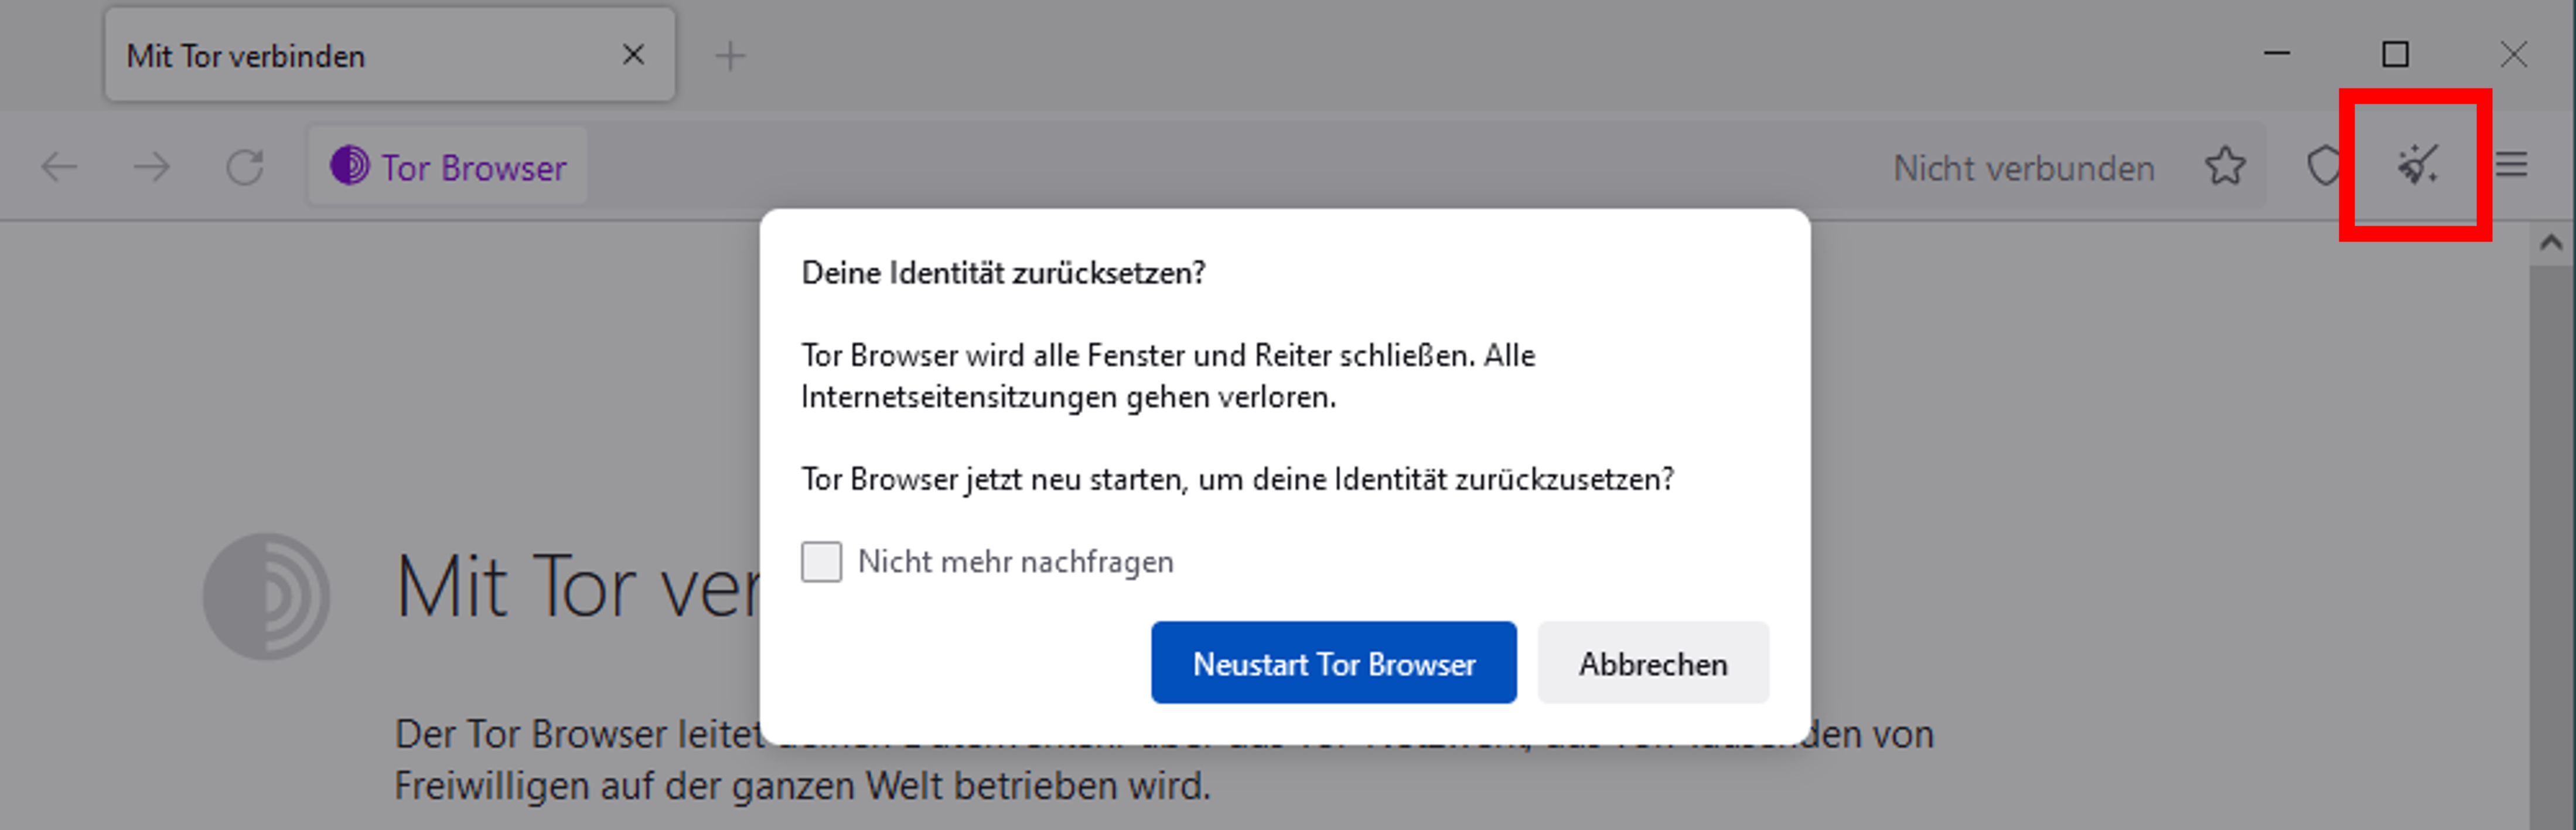
\includegraphics{bilder/tor-new-identity.png}}
		%	\label{...}
			\caption{Tabelle mit wiederherstellbaren Dateien: Logfile 1 vs. Logfile 2}
		\end{figure}
		- Tor hat die Funktion der "Neuen Identität" % https://support.torproject.org/de/glossary/new-identity/
			"Im Tor-Browser ermöglicht die "Neue Identität" eine schnelle und einfache Möglichkeit, Ihre Online-Identität zu ändern und Ihre Privatsphäre zu wahren. Wenn Sie den "Identitäts-Reset" im Tor-Browser durchführen, werden bestimmte Informationen und Daten gelöscht oder zurückgesetzt, um potenziell die Rückverfolgbarkeit Ihrer Online-Aktivitäten zu verringern."
			> Von Tor angegebene Auswirkungen:  alle deine geöffneten Tabs und Fenster geschlossen, alle privaten Informationen wie Cookies und Browserverlauf.
		- Deshalb: Bei Tor Daten zusätzlich vor und nach Neuer Identiät sammeln.
		\begin{figure}[h!]
			\centering
			\small
			\centerline{\resizebox{\linewidth}{!}{\input{bilder/datensammlung-zeitpunkte-tor-Latex.pdf_tex}}}
			\caption{Datensammlung Zeitpunkte Tor}
			\label{fig:jes}
		\end{figure}
	
	

\section{Datenanalyse}

> Analysis Stage (= Kapitel „Results“)
- Analyse der gesammelten Daten der vorherigen Phase: 
	> Process Monitor Logfiles	
	> Speicherabbilder: VM-Snapshots, RAM-Dumps
- Analyse heißt hier: Suchen nach PB Artefakten in gesammelten Daten
= Suchen Nach Strings, die einem Schritt im Browsing Szenario zugeordnet werden können
*** TODO: Liste von Strings ***

Wichtig dabei: (siehe Ziel der Arbeit): gefundenes Artefakt muss eindeutig Browser zugeordnet werden können.
Oft kritisiert: Viele Autoren verlassen sich beispielsweise bei der Analyse der RAM-Dumps auf eine einfache Stringsuche in einem Hexadezimal-Editor.
Sagt jedoch nichts darüber aus, ob gefundener String tatsächich auf privates Browsen zurückzuführen ist.
*** TODO: String in Editor Beispiel ***

Die gesammelten Daten dieses Versuchs lassen sich in drei Kategorien aufteilen:
> Common Locations
> Uncommon Locations	
> Registry

\subsection{Common Locations}

"Gängige Speicherorte beziehen sich auf die standardmäßigen Verzeichnisse oder Pfade, in denen bestimmte Dateien oder Informationen typischerweise in einem Betriebssystem oder einer Anwendung gespeichert werden."	
- auch "Vor-Ort-Triage" \cite{Horsman.2019} genannt, um bekannte Speicherorte nach PB Artefakte zu überprüfen
- z.B. Profile-Ordner von Browsern, wo Nutzerdaten gespeichert werden
- Befasst sich ausschließlich mit Dateien, die auf Festplatte geschrieben werden
- "Suchrichtung": Bekannte Browser-Speicherorte und Dateien -> Prüfen ob Dateien PB Artefakte enthalten
- Hier: Browser Speicherorte werden über die Schreiboperationen der Process Monitor Logfiles identifiziert 

Eng verwandt mit den "Common Locations" ist die "Whitebox-Analyse": (gezieltes Suchen nach Dateien) \cite{Bonetti.2014}
> Definition: "White-Box" Computer Forensik bezieht sich auf eine forensische Untersuchungsmethode, bei der der forensische Analyst über umfassende Kenntnisse und Zugriff auf das untersuchte System verfügt. Im Kontext der Computerforensik bezieht sich "White-Box" darauf, dass der Analyst über volle Transparenz und Zugriff auf alle Informationen, Ressourcen und Artefakte des Systems verfügt.
> Die "White-Box" Forensik kann verschiedene Techniken und Tools umfassen (z.B. Process Monitor, Regshot, Registry Explorer, Dekomprimierungstools), um Daten wiederherzustellen, gelöschte Informationen wiederherzustellen, Metadaten zu analysieren, Netzwerkaktivitäten zu überwachen und weitere forensische Analysen durchzuführen. Der Fokus liegt darauf, das System vollständig zu verstehen und alle relevanten Beweise zu sammeln.

\subsubsection*{Process Monitor Logfiles}

Grundlage für Common Locations = Process Monitor Logfiles

Datenaufbereitung für jede Logfile:
- Für Common Locations Filter setzen: 
	\begin{figure}[h!]
		\resizebox{\linewidth}{!}{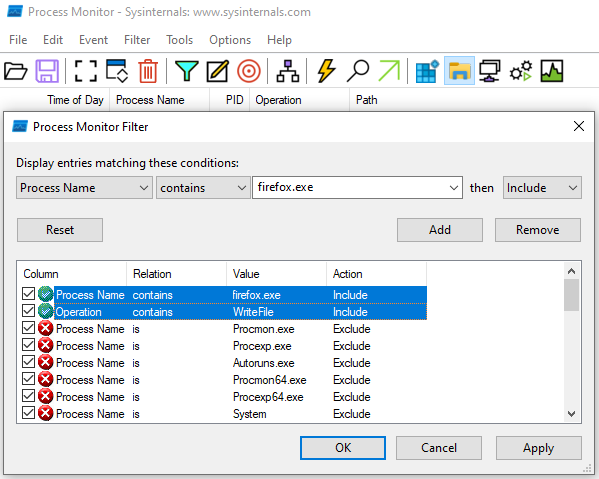
\includegraphics{bilder/process-monitor-filter.png}}
	%	\label{...}
		\caption{Tabelle mit wiederherstellbaren Dateien: Logfile 1 vs. Logfile 2}
	\end{figure}
	> Nur "File System Activity"
	> Process Name: contains "Browser-Prozess".exe
		- Firefox = firefox.exe
		- Tor = firefox.exe und tor.exe
		- Chrome = chrome.exe
		- Brave = brave.exe
	> Operation: contains "WriteFile"
- Gefiltertes Logfile als CSV exportieren, dann in Excel öffnen
- Irrelevante Spalten löschen: 
	> Time of Day
	> Process Name (Da in Process Monitor bereits nach Namen gefiltert wurde -> Alle Prozesse haben gleichen Namen)
	> Operation (Da in Process Monitor bereits nach Operation gefiltert wurde -> Alle Prozesse haben gleiche Operation „WriteFile“)
	> Result
	> Detail
- Gleiche Operationen (Duplikate) löschen
- Gruppieren nach browserspezifischen Speicherorten

Datenanalyse für jede geschriebene Datei:
I) Dateiextraktion
	1.	In Autopsy prüfen, ob Datei in Image von entsprechendem Snapshot vorhanden. Siehe Abbildung X: 
			> Logfile 1 -> Snapshot 2
			> Logfile 2 -> Snapshot 3
		Tor:
			> Logfile 1 -> Snapshot 2
			> Logfile 2-1 -> Snapshot 3-1
			> Logfile 2-2 -> Snapshot 3-2
	2.	Wenn ja, Dateien mit Autopsy extrahieren 
	3.	Wenn nein, prüfen, ob Datei in RAM gecacht:
		> Dazu Ausgabe von Volatiltiy Plugin "filescan" in entsprechendem RAM-Dump prüfen.
			> filescan: Das filescan-Plugin von Volatility durchsucht den Arbeitsspeicher nach Speicherbereichen, die Informationen über Dateien enthalten. Die Ausgabe des Plugins enthält eine Liste von Dateinamen, die im Speicher gefunden wurden. Können sein: Ausführbare Dateien, Bibliotheksdateien oder Konfigurationsdateien.
				% vol.py -f ram_dump.img windows.filescan > filescan.txt
		Welchen Dump bei welcher Logfile?
			> Logfile 1 -> RAM-Dump 2
			> Logfile 2 -> RAM-Dump 3
		Tor:
			> Logfile 1 -> RAM-Dump 2
			> Logfile 2-1 -> RAM-Dump 3-1
			> Logfile 2-2 -> RAM-Dump 3-2
		> Wenn Datei gefunden wurde: Datei mit dumpfiles und entsprechender virtueller Dateispeicheradresse extrahieren.
		\begin{figure}[h!]
			\centering
			\small
			\centerline{\resizebox{\linewidth}{!}{\input{bilder/volatility-filescan-dumpfiles-Latex.pdf_tex}}}
			\caption{Datensammlung Zeitpunkte Tor}
			\label{fig:jes}
		\end{figure}
	4. Wenn Datei auch nicht im RAM gecacht ist: Prüfen, ob es sich bei Datei um Hilfsdatei handelt. Dabei handelt es sich meistens um temporäre Dateien mit zusätzlicher Dateiendung (meistens .tmp)
	5. Wenn ja: Zur die Dateiendung der Hilfsdatei weglassen und bei Schritt 1 beginnen. z.B: Wenn Datei "some-file.json.tmp" nicht existiert, prüfen, ob Datei "some-file.json" existiert
	6. Wenn nein: Datei als "nicht wiederherstellbar" markieren
II) Dateianalsye (nachdem Datei extrahiert wurde)
	7. Datei mit entsprechdem Tool untersuchen 
	8. Wenn Datei nicht direkt untersuchbar ist: ggf. Mit zusätzlichem Tool Datei vorberarbeiten. z.B. Wenn es sich um komprimierte Dateien handelt
	9. In Excel-Tabelle markieren, ob Datei PB Artefakte enthält. Dabei gibt es drei Zustände: 
		- leere Datei
		- neuer (nicht-leerer) Inhalt
		- gleichbleibender Inhalt
	\begin{figure}[h!]
		\centering
		\small
		\centerline{\resizebox{\linewidth}{!}{\input{bilder/process_monitor_to_exce-Latexl.pdf_tex}}}
		\caption{TODO: Process Monitor Write Operation to Excel Spreadsheet}
		\label{fig:jes}
	\end{figure}

\subsubsection*{SQLite-Datenbänke}
- Besondere Rolle nehmen bei den ausgewählten Browsern SQLite Datenbänke ein.

"SQLite-Datenbanken sind besonders wichtig bei Webbrowsern wie Firefox, Tor, Chrome und Brave, da sie Informationen wie Lesezeichen, Browserverlauf, Caches, Cookies und Erweiterungsdaten speichern. Diese Datenbanken bieten Benutzern eine personalisierte Browsererfahrung und sind für Forensiker und Sicherheitsexperten von Bedeutung, um relevante Informationen über die Online-Aktivitäten eines Benutzers zu analysieren."

"Die Verwendung von SQLite-Datenbanken in diesen Webbrowsern bietet Effizienz, Flexibilität und eine einfache Möglichkeit, Daten zu organisieren und abzurufen. Für Forensiker und Sicherheitsexperten sind diese Datenbanken von Bedeutung, da sie wertvolle Informationen über die Online-Aktivitäten eines Benutzers enthalten können, die bei Untersuchungen, Sicherheitsanalysen oder forensischen Untersuchungen relevant sein können."

> Deshalb: Für jeden Browser werden die SQLite Datenbanken in allen Snapshots miteinander verglichen.
\begin{figure}[h!]
	\centering
	\small
	\centerline{\resizebox{\linewidth}{!}{\input{bilder/sqlite-methodology-Latex.pdf_tex}}}
	\caption{TODO: Process Monitor Write Operation to Excel Spreadsheet}
	\label{fig:jes}
\end{figure}
I) Dateiextraktion analog zu Dateien im Process Monitor
II) Dateianalyse:
	- SQLite Datenbank wird mit gleicher SQLite Datenbank aus vorherigem Snapshot verglichen (wenn vorhanden) -> Unterschiede in Excel-Tabelle festgehalten
	- Wichtig: Zu jeder SQLite Datenbank gibt es normalerweise eine .sqlite-wal Datei. 
		"Die Dateien mit der Erweiterung ".sqlite-wal" sind WAL-Dateien (Write-Ahead Log) in Verbindung mit SQLite-Datenbanken. Sie werden von SQLite verwendet, um Änderungen an einer Datenbank vorübergehend zu protokollieren, bevor sie dauerhaft in die Hauptdatenbankdatei geschrieben werden. Die WAL-Dateien dienen als Transaktions-Log und ermöglichen eine effiziente und sichere Aktualisierung der SQLite-Datenbanken, insbesondere in Situationen mit gleichzeitigen Schreibvorgängen."
		> Inhalte werden erst in WAL Datei geschrieben, dann in SQLite Datei
	- Deshalb: WAL Änderungen in SQLite Datei schreiben, danach sqldiff mit gleicher Datenbank ohne WAL Änderungen -> Unterschiede in Excel-Tabelle
		1) über sqlite3 Kommandozeile .sqlite Datenbank öffnen: % sqlite3 <Datenbank>.sqlite
		2) Über Pragma Befehl WAL Checkpoint durchführen: % sqlite3> PRAGMA wal_checkpoint;

\subsection{Uncommon Locations}

"Ungewöhnliche Speicherorte beziehen sich auf Verzeichnisse oder Orte, die nicht zu den gängigen oder standardmäßigen Speicherorten gehören."
= „Unbekannte Speicherorte“, nur durch tiefgehende forensische Analyse entdeckt
Blackbox-Analyse: \cite{Bonetti.2014} (Stringsuchen im gesamten Image mithilfe von Tool) 
= Durchsuchung des Beweismaterials ohne Vorwissen über Browserverhalten (d.h. welche Dateien geschrieben wurden) sowie ohne Vorverarbeitung der Dateien (z.B. Entpacken von Dateien).
Stattdessen: Untersuchen der Images nur mittels vordefinierter Funktionen von Forensik-Tools, da dies schnelles erstes Mittel von Forensikern, um nach Acquisition Phase Ergebnisse zu erhalten
- wichtigster Unterschied zu "Common Locations": Umgekehrte Suchrichtung => PB Artefakt (String) -> Alle Daten nach PB Artefakt durchsuchen
- Eigenschaften:
	> Wenn manuell durchgeführt, deutlich Zeitaufwändiger
	> Deshalb: Unterstützung durch Forensik-Tools. 
	> Vertrauen in die Vollständigkeit der Tools
- Beispiele in der Literatur:
	> “\$MFT”, “\$LogFile”, “Favicons”, “etilqs”, “Manifest.json”, “pagefile.sys.”, “unallocated space” and “slack space” \cite{Montasari.2015}	

Bei Browser Forensik hier oft verwendet: Stichwortsuchen über gesamtes Speicherabbild

Wichtig: String-Treffer muss Browser zugeordnet werden können
> Oft wiederkehrende Negativbeispiele in Literatur: gesamten RAM-Dump in Hexadezimaleditor geöffnet, danach: Stringsuche nach PB Artefakten. \cite{Rochmadi.2017, Md.2018, Montasari.2015}
> Problem: Gefundener String kein Indiz, dass tatsächlich Artefakt in Zusammenhang mit PB aufgetaucht ist.
> Gegenbeispiel: String in Textdatei in Desktop speichern. RAM Dump enthält String.

\subsubsection*{Analyse mit Autopsy}

Bei White-Box Analyse: Autopsy nur zur Dateiextraktion genutzt, hier: als konkretes forensisches Werkzeug

> Stichwortsuche über gesamtes Festplatten-Image
	*** TODO: Screenshot von Suchfunktion ***
> Zusätzlich: Autopsy PlugIns indexieren und kategoriesieren bereits Dateien
	- Web Bookmarks
	- Web Cookies
	- Web History
	- Web Categories

\subsubsection*{Analyse mit Volatility}

Bei White-Box Analyse: Volatility nur zur Dateiextraktion genutzt, hier: als konkretes forensisches Werkzeug

Wie oben ausführlich beschrieben: gefundener String im RAM muss Browser zugeordnet werden können -> Passendes Werkzeug = Volatility PlugIn "Yarascan". (siehe Kapitel Analysewerkzeuge)

*** TODO: konkrete Yara-Rules hier einfügen ***
> HTML-Fragmente: \cite{Said.2011} 
> Image als Hex: \cite{Ohana.2013}

> yarascan: Das Plugin "yarascan" ermöglicht die Durchführung einer YARA-basierten Malware-Erkennung im Arbeitsspeicherabbild. YARA ist eine flexible Regel-Engine, die verwendet werden kann, um nach bestimmten Mustern, Signaturen oder Verhaltensmerkmalen von Malware zu suchen. Das Plugin wendet YARA-Regeln auf den Arbeitsspeicher an und gibt potenzielle Treffer aus.
		% vol.py -f ram_dump.img windows.vadyarascan --yara-file yara_rules.yara > yarascan.txt
		Wichtig: yara\_rules.yara = In domainspecific Yara-Skriptsprache geschriebene Regeln, nach welchen RAM durchsucht wird.
		Hier: Einfache String-Pattern, die jeden Schritt des Browsing-Szenarios abdecken:
		*** TODO Beispielhafte Yara-Rules einfügen ***
		*** TODO: Erklärung Yara-Ausgaben, mit Screenshot ***
	=> Wichtig hier: Gibt PID des Prozesses und virtuelle Adresse des gefundenen Strings im Speicherbereich des Prozesses an

> Davon ausgehend: pslist: 
Das Plugin "pslist" wird verwendet, um eine Liste der aktiven Prozesse im Arbeitsspeicherabbild zu erstellen. Es extrahiert Informationen wie Prozessnamen, PID (Prozess-ID), Elternprozess, Startzeitpunkt, Priorität und andere Attribute für jeden laufenden Prozess.
		% vol.py -f ram_dump.img windows.pslist > pslist.txt
	=> Wichtig hier: Prozessname 	

> "String Kontext" herausfinden = Prüfen, ob in Speicherseite  über und unter gefundenen String weitere Zusammenhänge zu erkennen sind.
> Dazu: memmap: 
Das Plugin "memmap" dient dazu, eine detaillierte Karte des physischen Speichers des Systems zu erstellen. Es gibt Informationen über die physischen Speicherbereiche, deren Startadressen, Größen, Schutzattribute und andere relevante Details. Dieses Plugin kann bei der Analyse von Speicherlayout und -nutzung hilfreich sein.
		1) % vol.py -f ram_dump.img windows.memmap --pid <PID> > memmap.txt
			gibt Abbildung der Adressen des virtuellen Speichers auf die physikalische Adresse des Speicherbereichs des Prozesses mit der PID <PID>.
			Weiterhin und hier relevant: gibt Abbildung von virtuellen Adresse auf einen Datei-Offset an. Dieser bezieht sich auf die Datei, die erzeugt wird, wenn der Befehl mit dem --dump Flag ausgeführt wird:
		2) % vol.py -f ram_dump.img -o \dump_dir\ windows.memmap --pid <PID> --dump
			führt dies zur physischen Extraktion des Speicherbereichs des Prozesses mit der PID <PID> in eine separate Datei.		
 => Extrahierte Seite mit Hexeditor HxD untersuchen

\begin{figure}[h!]
	\centering
	\small
	\centerline{\resizebox{\linewidth}{!}{\input{bilder/yarascan_plugin_tree-Latex.pdf_tex}}}
	\caption{TODO: Process Monitor Write Operation to Excel Spreadsheet}
	\label{fig:jes}
\end{figure}


\subsection{Registry}
- zählt sowohl Common als auch Uncommon Location -> Deshalb eigene Kategorie
- Common: Analyse der Process Monitor Schreiboperationen in Registry
	Datenaufbereitung für jede Logfile:
	- Grundlage = Process Monitor Logfiles
	- Für Common Locations Filter setzen: 
		\begin{figure}[h!]
			\resizebox{\linewidth}{!}{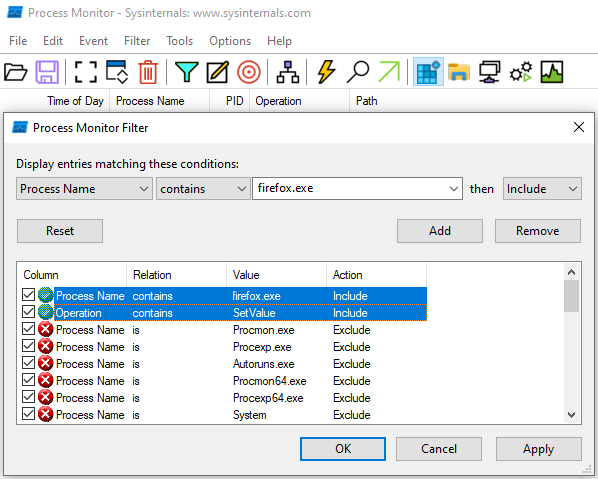
\includegraphics{bilder/process-monitor-filter-registry.png}}
		%	\label{...}
			\caption{Tabelle mit wiederherstellbaren Dateien: Logfile 1 vs. Logfile 2}
		\end{figure}	
		> Nur "Registry Activity"
		> Process Name: contains "Browser-Prozess".exe
			- Firefox = firefox.exe
			- Tor = firefox.exe und tor.exe
			- Chrome = chrome.exe
			- Brave = brave.exe
		> Operation: contains "SetValue"
	- Gefiltertes Logfile als CSV exportieren, dann in Excel öffnen
	- Gleiche Operationen (Duplikate) löschen
	- Browserspezifisches Gruppieren 
	Datenanalyse für jeden geschriebenen Registry Key: Value untersuchen (steht in CSV hinter jeder Key Schreiboperation)
	

- Uncommon: Stringsuche in bekannten Registry Hives mit Registry Explorer

	"Ein Registry Hive ist eine Datei in der Windows-Registry, die als Container für spezifische Arten von Konfigurations- und Nutzerdaten dient. Jedes Hive hat eine bestimmte Funktion, wie die Speicherung von Systemeinstellungen (System-Hives) oder individuellen Benutzerkonfigurationen (User-Hives). Die Hives im System32\\Config-Verzeichnis enthalten wichtige Informationen für das Betriebssystem, während die User-Hives unter dem jeweiligen Benutzerverzeichnis gespeichert werden. Diese Hives werden von Windows beim Start geladen und dienen als Quelle für Einstellungen und Informationen, die von verschiedenen Systemkomponenten und Anwendungen genutzt werden."	

	Quelle für Hives: % https://medium.com/@haircutfish/tryhackme-windows-forensics-1-task-3-accessing-registry-hives-offline-task-4-data-acquisition-b440f5be2a13
	
	System-Hives im Verzeichnis "% C:\Windows\System32\Config":
	===========================
    DEFAULT: Enthält die Standardkonfigurationseinstellungen für neue Benutzerprofile.
    SAM: Enthält die Sicherheitskontenverwaltungsdaten, einschließlich der Benutzerkonten und deren Kennwörter.
    SECURITY: Enthält Sicherheitsinformationen, die für die Zugriffssteuerung und Authentifizierung verwendet werden.
    SOFTWARE: Enthält Konfigurationsdaten für installierte Software und Anwendungen.
    SYSTEM: Enthält Systemkonfigurationseinstellungen und Gerätetreiberinformationen.

	User-Hives im Verzeichnis "% C:\Users<username>":
	=========================
    NTUSER.DAT: Enthält die individuellen Einstellungen und Konfigurationen für den angemeldeten Benutzer. 
    USRCLASS.DAT: Enthält Informationen über die Dateizuordnungen und Registrierungseinstellungen für den angemeldeten Benutzer im Zusammenhang mit seinen benutzerdefinierten Klassen. 

	Analyse der Hives für jeden VM-Snapshot: Alle Hives in eine Registry Explorer Sitzung, danach Stringsuche nach PB Artefakten	

